\documentclass[10pt]{beamer}

% ------------------------------------------------------------------------
% Carga de tu preámbulo personalizado (preamble.tex).
% Recuerda colocarlo en la misma carpeta para que \input funcione.
% ------------------------------------------------------------------------
\usetheme[progressbar=frametitle]{metropolis}
\usepackage{appendixnumberbeamer}
\usepackage{fancyvrb}
\usepackage{booktabs}
\usepackage[scale=2]{ccicons}
\usepackage{pgfplots}
\usepgfplotslibrary{dateplot}
\usepackage{type1cm}
\usepackage{lettrine}
\usepackage{ragged2e}
\usepackage{xspace}
\newcommand{\themename}{\textbf{\textsc{metropolis}}\xspace}
\usepackage{graphicx} % Allows including images
\usepackage{booktabs} % Allows the use of \toprule, \midrule and \bottomrule in tables
\usepackage[utf8]{inputenc} %solucion del problema de los acentos.
\usepackage{xcolor}
\definecolor{LightGray}{gray}{0.9}

\usepackage{minted}
\usemintedstyle{tango}
\newcommand{\mypyfile}[1]{\inputminted[linenos=true, fontsize=\footnotesize, frame=lines, framesep=5\fboxrule,framerule=1pt]{python}{#1}}

\setminted[python]{breaklines,frame=lines,framesep=2mm,baselinestretch=1.2,bgcolor=LightGray,linenos, fontsize=\footnotesize} % obeytabs=true, tabsize=2, showtabs=true}

%%%%%%%%%%%%%%%%%%%%%%%%%%%%%%%%%%%%%%%%%%%%%%%%%%%%%%%%%%%%%%%%%%%%%%%%%%%%%%%%%%%%%%
\setbeamercolor{progress bar}{fg=blue!50!black,bg=white!50!black}
\setbeamercolor{title separator}{fg=red!50!black,bg=white!50!black}
\setbeamercolor{frametitle}{fg=white!80!black,bg=red!50!black}
\title[PCFI161]{Programaci\'on para F\'isica y Astronom\'ia}
\subtitle{Departamento de Física.}

\newcommand{\myfront}{
\author[PCFI161]{Corodinadora: C Loyola \\ Profesoras/es C Loyola / C Femenías / Y Navarrete / C Ruiz}
\institute[UNAB]{Universidad Andrés Bello}
\date{Primer Semestre 2025}
}

\titlegraphic{%
  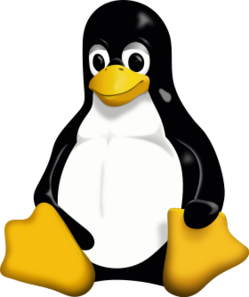
\includegraphics[width=.08\textwidth]{logo-tux.png}\hfill
  
\includegraphics[width=.3\textwidth]{logo-unab.png}\hfill
  
\includegraphics[width=.08\textwidth]{logo-python.png}
}

\makeatletter
\setbeamertemplate{title page}{
  \begin{minipage}[b][\paperheight]{\textwidth}
    \vfill%
    \ifx\inserttitle\@empty\else\usebeamertemplate*{title}\fi
    \ifx\insertsubtitle\@empty\else\usebeamertemplate*{subtitle}\fi
    \usebeamertemplate*{title separator}
    \ifx\beamer@shortauthor\@empty\else\usebeamertemplate*{author}\fi
    \ifx\insertdate\@empty\else\usebeamertemplate*{date}\fi
    \ifx\insertinstitute\@empty\else\usebeamertemplate*{institute}\fi
    \vfill
    \ifx\inserttitlegraphic\@empty\else\inserttitlegraphic\fi
    \vspace*{1cm}
  \end{minipage}
}
\makeatother


\makeatletter
\setlength{\metropolis@titleseparator@linewidth}{2pt}
\setlength{\metropolis@progressonsectionpage@linewidth}{2pt}
\setlength{\metropolis@progressinheadfoot@linewidth}{2pt}
\makeatother


\begin{document}

% ------------------------------------------------------------------------
% Portada de la Presentación
% ------------------------------------------------------------------------
\myfront{}

% ------------------------------------------------------------------------
% Slide 1: Título de la Sesión
% ------------------------------------------------------------------------
\begin{frame}
  \titlepage
  % Por ejemplo:
  % \title{Semana 10 - Sesión 1 (Sesión 19): Repaso Integral y Ejercicios Previos a Solemne II}
\end{frame}

% ------------------------------------------------------------------------
% Slide 2: Índice / Tabla de contenidos
% ------------------------------------------------------------------------
\begin{frame}
  \frametitle{Resumen - Semana 10, Sesión 1 (Sesión 19)}
  \tableofcontents
\end{frame}

% ------------------------------------------------------------------------
% Configuración de bloques
% ------------------------------------------------------------------------
\metroset{block=fill}

% ----------------------------------------------------------------------------------------
% SECCIÓN 1: Introducción y Conexión con Sesiones Previas
% ----------------------------------------------------------------------------------------
\section{Introducción y Contexto}

% ------------------------------------------------------------------------
% Slide 3: Repaso de Semanas Anteriores
% ------------------------------------------------------------------------
\begin{frame}{Repaso de las Semanas 8 y 9}
  \begin{itemize}
    \item \textbf{Semana 8}:
      \begin{itemize}
        \item \textbf{POO básica} (clases, atributos, métodos, \_\_init\_\_).
        \item Integración con NumPy/pandas para datos, problemas evaluados.
      \end{itemize}
    \item \textbf{Semana 9}:
      \begin{itemize}
        \item \textbf{Herencia}, métodos especiales (\_\_str\_\_, \_\_repr\_\_).
        \item Ejercicios sobre \textbf{Body/Star}, \textbf{Particle/ChargedParticle}, etc.
        \item También tuvimos evaluaciones parciales en grupos (POO + datos).
      \end{itemize}
    \item \textbf{Objetivo de hoy}: Repasar de forma integral todos los contenidos recientes, resolver ejercicios previos a la \textbf{Solemne II} (próxima sesión).
  \end{itemize}
\end{frame}

% ------------------------------------------------------------------------
% Slide 4: Objetivos de la Sesión 19
% ------------------------------------------------------------------------
\begin{frame}{Objetivos de la Sesión 19}
  \begin{itemize}
    \item \textbf{Revisar} y \textbf{ejercitar} los conceptos clave:
      \begin{itemize}
        \item POO (clases, herencia, métodos).
        \item NumPy avanzado (manipulación de arreglos, linalg).
        \item Matplotlib (subplots, histogramas, 3D).
        \item pandas (lectura de CSV, manejo de DataFrame básico).
      \end{itemize}
    \item \textbf{Resolver} ejercicios integrales que unan estos temas.
    \item \textbf{Prepararnos} para la \textbf{Solemne II} (Semana 10, Sesión 2), revisando dudas y áreas de dificultad.
  \end{itemize}
\end{frame}

% ----------------------------------------------------------------------------------------
% SECCIÓN 2: Resumen de Contenidos Clave
% ----------------------------------------------------------------------------------------
\section{Resumen de Contenidos Clave}

% ------------------------------------------------------------------------
% Slide 5: POO (Repaso Rápido)
% ------------------------------------------------------------------------
\begin{frame}{POO: Claves a Recordar}
  \begin{itemize}
    \item \textbf{Clases} y \textbf{Objetos}: \(\texttt{class Nombre}:\) y \(\texttt{obj = Nombre(...)}\).
    \item \textbf{\_\_init\_\_ (constructor)} para inicializar atributos.
    \item \textbf{Herencia}: \(\texttt{class Derivada(BaseClass):} ... \texttt{super().\_\_init\_\_}\).
    \item Métodos especiales: \(\texttt{\_\_str\_\_}\), \(\texttt{\_\_repr\_\_}\), etc.
    \item Ejemplos: \(\texttt{Particle}\), \(\texttt{ChargedParticle}\), \(\texttt{Body}\), \(\texttt{Star}\).
  \end{itemize}
\end{frame}

% ------------------------------------------------------------------------
% Slide 6: NumPy Avanzado
% ------------------------------------------------------------------------
\begin{frame}{NumPy: Claves a Recordar}
  \begin{itemize}
    \item \textbf{ndarray} con creación (\texttt{np.array}), \texttt{zeros}, \texttt{ones}, \texttt{arange}, \texttt{linspace}.
    \item \textbf{reshape}, \texttt{transpose}, \texttt{concatenate} (hstack, vstack).
    \item \textbf{np.random} (valores aleatorios), \textbf{np.linalg} (inversa, determinante, eigenvalores).
    \item Broadcasting y operaciones vectorizadas (suma, resta, multiplicación, etc. sin bucles).
  \end{itemize}
\end{frame}

% ------------------------------------------------------------------------
% Slide 7: Matplotlib
% ------------------------------------------------------------------------
\begin{frame}{Matplotlib: Claves a Recordar}
  \begin{itemize}
    \item \(\texttt{plt.plot(x, y)}\), \(\texttt{plt.scatter()}\), \(\texttt{plt.hist()}\), \(\texttt{plt.bar()}\).
    \item \(\texttt{subplots()}\) para múltiples paneles (axs).
    \item Gráficos \textbf{3D} con \(\texttt{Axes3D}\) o \(\texttt{subplots(projection='3d')}\).
    \item Personalización: \(\texttt{xlabel, ylabel, title, legend, colorbar}\).
    \item \(\texttt{plt.tight\_layout()}\) para ajustar márgenes.
  \end{itemize}
\end{frame}

% ------------------------------------------------------------------------
% Slide 8: pandas
% ------------------------------------------------------------------------
\begin{frame}{pandas: Claves a Recordar}
  \begin{itemize}
    \item \(\texttt{import pandas as pd}\).
    \item Lectura de CSV: \(\texttt{df = pd.read\_csv("archivo.csv")}\).
    \item \(\texttt{df.head()}\), \(\texttt{df.describe()}\), \(\texttt{df.columns}\).
    \item Selección de columnas: \(\texttt{df['col']}\), \(\texttt{df[['col1','col2']]}\).
    \item Iteración de filas: \(\texttt{df.iterrows()}\) o \(\texttt{df.itertuples()}\).
    \item Integración con \textbf{NumPy} y \textbf{Matplotlib} para análisis y graficación.
  \end{itemize}
\end{frame}

% ----------------------------------------------------------------------------------------
% SECCIÓN 3: Ejercicios de Repaso
% ----------------------------------------------------------------------------------------
\section{Ejercicios de Repaso}

% ------------------------------------------------------------------------
% Slide 9: Ejercicio 1 - POO + NumPy (Matrices)
% ------------------------------------------------------------------------
\begin{frame}{Ejercicio 1: Clase y Matriz de Distancias}
  \begin{block}{Enunciado}
    \begin{itemize}
      \item Crear una clase \(\texttt{Point}\) con atributos (\texttt{name, x, y}).
      \item Método \(\texttt{distance(self, other)}\) que devuelva \(\sqrt{(x1-x2)^2 + (y1-y2)^2}\).
      \item Instanciar 5 objetos \(\texttt{Point}\) (pueden ser aleatorios).
      \item Crear \(\texttt{np.zeros((5,5))}\) y rellenar con las distancias entre cada par de \(\texttt{Point}\).
      \item Visualizar la matriz en \(\texttt{plt.imshow}\) con \(\texttt{colorbar()}\).
    \end{itemize}
  \end{block}
  \textbf{Objetivo}: Reforzar \textbf{clase simple}, \textbf{distancia} y \textbf{matriz NxN} con NumPy + visualización.
\end{frame}

% ------------------------------------------------------------------------
% Slide 10: Ejercicio 2 - Herencia y Gráfica
% ------------------------------------------------------------------------
\begin{frame}{Ejercicio 2: Partículas con Herencia}
  \begin{block}{Enunciado}
    \begin{itemize}
      \item Crear clase base \(\texttt{Particle}\) con (\texttt{mass, x, y}) y método \(\texttt{kinetic\_energy(vx,vy)}\).
      \item Crear clase derivada \(\texttt{ChargedParticle}\) con \texttt{charge} y método \(\texttt{potential\_energy(E\_field)}\).
      \item Instanciar 3-4 \(\texttt{ChargedParticle}\) con datos aleatorios (usando \texttt{np.random}).
      \item Graficar \(\textbf{scatter}\) en 2D (eje X, Y) coloreado según \(\texttt{charge}\) (p. ej. \texttt{c=charge} + colormap).
      \item Mostrar \(\textbf{title}\), \(\textbf{xlabel}\), \(\textbf{ylabel}\).
    \end{itemize}
  \end{block}
  \textbf{Objetivo}: Reforzar \textbf{herencia}, uso de \textbf{np.random} y \textbf{scatter} con color mapping.
\end{frame}

% ------------------------------------------------------------------------
% Slide 11: Ejercicio 3 - pandas CSV y Subplots
% ------------------------------------------------------------------------
\begin{frame}{Ejercicio 3: DataFrame, Análisis y Subplots}
  \begin{block}{Enunciado}
    \begin{itemize}
      \item Suponiendo un CSV (\texttt{measurements.csv}) con columnas \(\texttt{name, value, category}\).
      \item Cargar con \(\texttt{pandas.read\_csv}\).
      \item Crear un \textbf{subplot con 2 paneles}:
        \begin{itemize}
          \item Panel 1: \textbf{histograma} de la columna \texttt{value}.
          \item Panel 2: \textbf{barra} de \texttt{value} por \texttt{name}, separando o coloreando por \(\texttt{category}\) (si cabe).
        \end{itemize}
      \item Mostrar \(\texttt{df.describe()}\) para ver estadísticas rápidas.
    \end{itemize}
  \end{block}
  \textbf{Objetivo}: Integrar \textbf{pandas} (lectura + describe) con \textbf{subplots} de Matplotlib.
\end{frame}

% ------------------------------------------------------------------------
% Slide 12: Ejercicio 4 (Opcional) - POO y pandas
% ------------------------------------------------------------------------
\begin{frame}{Ejercicio 4 (Opcional): Cargar Objetos desde CSV}
  \begin{block}{Enunciado}
    \begin{itemize}
      \item CSV con \(\texttt{name, mass, charge, x, y}\).
      \item Clase \texttt{ChargedParticle} (hereda de \(\texttt{Particle}\)).
      \item Iterar filas del DF para instanciar objetos en una lista \(\texttt{particles}\).
      \item Calcular la energía cinética total asumiendo \(\texttt{vx, vy}\) aleatorios o fijos.
      \item \textbf{Visualizar} la distribución de \(\texttt{charge}\) en un histograma.
    \end{itemize}
  \end{block}
  \textbf{Objetivo}: Profundizar la \textbf{creación masiva} de objetos con datos CSV, combinando \textbf{NumPy} y \textbf{Matplotlib}.
\end{frame}

% ----------------------------------------------------------------------------------------
% SECCIÓN 4: Actividad en Clase
% ----------------------------------------------------------------------------------------
\section{Actividad en Clase}

% ------------------------------------------------------------------------
% Slide 13: Trabajo Colaborativo
% ------------------------------------------------------------------------
\begin{frame}{Trabajen en Grupos}
  \begin{itemize}
    \item \textbf{Parejas o tríos}, elijan 2+ ejercicios o combínenlos.
    \item \textbf{Objetivo}: Repasar antes de la Solemne II.
    \item Pueden usar \textbf{Colab} o local, comentando sus pasos y mostrando resultados (gráficas, matrices).
    \item Comparen resultados y listas de \textbf{dudas} para plantearlas al final.
  \end{itemize}
\end{frame}

% ------------------------------------------------------------------------
% Slide 14: Sugerencias Prácticas
% ------------------------------------------------------------------------
\begin{frame}{Sugerencias Prácticas}
  \begin{itemize}
    \item Revisen \textbf{módulos} importados: \(\texttt{import numpy as np}\), \(\texttt{import matplotlib.pyplot as plt}\), \(\texttt{import pandas as pd}\).
    \item Prueben \textbf{logging} básico o \textbf{print debugging} si algo sale mal.
    \item Usen \(\textbf{super()}\) y verifiquen si \(\textbf{\_\_str\_\_}\) es útil para imprimir objetos.
    \item Si hacen \textbf{matrices NxN}, consideren \(\texttt{np.fill\_diagonal(mat, 0)}\) para poner ceros en la diagonal, si es relevante.
  \end{itemize}
\end{frame}

% ------------------------------------------------------------------------
% Slide 15: Espacio para Dudas
% ------------------------------------------------------------------------
\begin{frame}{Espacio para Dudas Generales}
  \begin{itemize}
    \item ¿Preguntas sobre POO, herencia, métodos especiales?
    \item ¿Dificultades con \textbf{np.linalg} o \textbf{numpy.random}?
    \item ¿Matplotlib subplots, 3D, personalización?
    \item \(\textbf{pandas}\): \textbf{df.describe}, \textbf{df.iterrows}, merges, etc.
  \end{itemize}
  \vspace{0.3cm}
  \textbf{Levanten la mano para aclarar cualquier duda.}
\end{frame}

% ----------------------------------------------------------------------------------------
% SECCIÓN 5: Conclusiones y Preparación para Solemne II
% ----------------------------------------------------------------------------------------
\section{Conclusiones y Preparación}

% ------------------------------------------------------------------------
% Slide 16: Discusión de Soluciones
% ------------------------------------------------------------------------
\begin{frame}{Discusión de Soluciones}
  \begin{itemize}
    \item Compartan cómo resolvieron \textbf{distancias NxN}, \textbf{scatter con color}, \textbf{subplots}, etc.
    \item Si usaron \textbf{pandas}, ¿cómo filtraron datos o manipularon columnas?
    \item ¿Qué inconvenientes aparecieron en la parte POO?  
  \end{itemize}
\end{frame}

% ------------------------------------------------------------------------
% Slide 17: Conclusiones de la Sesión 19
% ------------------------------------------------------------------------
\begin{frame}{Conclusiones de la Sesión 19}
  \begin{itemize}
    \item Repasamos de forma integral \textbf{POO}, NumPy, Matplotlib y pandas con ejercicios.
    \item Identificamos \textbf{dudas} y resolvimos problemas típicos.
    \item Todo esto apunta a la \textbf{Solemne II} (próxima sesión), donde se evaluarán estos bloques de contenidos.
  \end{itemize}
\end{frame}

% ------------------------------------------------------------------------
% Slide 18: Preparándonos para la Solemne II
% ------------------------------------------------------------------------
\begin{frame}{Preparación para la Solemne II (Semana 10, Sesión 2)}
  \begin{itemize}
    \item \textbf{Revisar} apuntes y ejercicios hechos:
      \begin{itemize}
        \item Sintaxis de \textbf{class}, herencia, \_\_init\_\_, \_\_str\_\_.
        \item Principales funciones NumPy: \(\texttt{reshape}, \texttt{random}, \texttt{linalg}\).
        \item \(\textbf{Matplotlib}\): subplots, scatter, hist, 3D, personalización básica.
        \item \(\textbf{pandas}\) para CSV y df.plot (opcional).
      \end{itemize}
    \item \textbf{Practicar} resolviendo miniproblemas con tiempo.
    \item Cualquier duda final, ¡pregunten vía foros o en la próxima clase (antes de la Solemne)! 
  \end{itemize}
\end{frame}

% ------------------------------------------------------------------------
% Slide 19: Recursos Adicionales
% ------------------------------------------------------------------------
\begin{frame}{Recursos Adicionales}
  \begin{itemize}
    \item \href{https://docs.python.org/3/tutorial/classes.html}{\textbf{Python Tutorial - Clases}} (Repaso POO).
    \item \href{https://numpy.org/doc/}{\textbf{NumPy Docs}} (subsecciones de random, linalg).
    \item \href{https://matplotlib.org/stable/}{\textbf{Matplotlib Docs}} - Ejemplos de subplots y 3D.
    \item \href{https://pandas.pydata.org/}{\textbf{pandas Docs}} - sección de 10 minutes to pandas.
  \end{itemize}
\end{frame}

% ------------------------------------------------------------------------
% Slide 20: Cierre de la Sesión
% ------------------------------------------------------------------------
\begin{frame}
  \Huge{\centerline{¡Muchas gracias y éxito en su práctica!}}
  \vspace{0.3cm}
  \normalsize
  \begin{itemize}
    \item Recuerden estudiar para la \textbf{Solemne II} (Semana 10, Sesión 2).
    \item Cualquier duda, sigan participando en foros o consultas.
    \item ¡Nos vemos en la próxima sesión con la evaluación!
  \end{itemize}
\end{frame}

\end{document}

